\section{Checking Balance}
\label{sec:balance}

\subsection{Quick Overview}

In \MatchIt, there are two ways to check balance after any matching
procedure: numerical and graphical summaries. Both methods are based
on the idea summarized in Section~\ref{sec:balance-sum} and fully
described in \citet*{HoImaKin05}. Given the \MatchIt\ output object
{\tt m.out}, one can use the following commands,
\begin{enumerate}
\item \texttt{summary(m.out)} gives numerical summaries of the
  resulting balance of the covariates.
  
\item \texttt{plot(m.out)} gives graphical summaries to assess the
  balance of the covariates.
\end{enumerate}
Below, we give three examples (exact matching, nearest neighbor
matching, and subclassification) to illustrate the use of these two
functions. The same two commands can be used for all other matching
procedures, and they will give similar outputs.  See
Section~\ref{sec:outputs} for more details.


\subsection{Details}


\subsubsection{The {\tt summary()} Command}

The \texttt{summary()} command first gives measures of the balance
between the treated and control groups in the full (original) data
set, and then the same measures of balance in the matched data set.
If the matching worked well, the measures of balance should be smaller
in the matched data set as compared with the full data set.  The
specific balance measures given are described below.

The \texttt{summary()} output for subclassification is the same as
that for other types of matching, except that the balance statistics
are shown separately for each subclass, and the overall balance in the
matched samples is calculated by aggregating across the subclasses,
where each subclass is weighted by the number of units in the
subclass.  For exact matching, the covariate values within each
subclass are guaranteed to be the same, and so the measures of balance
are not output for exact matching; only the sample sizes in each
subclass are shown.

\begin{itemize}
\item {\bf Balance statistics:} The statistics the \texttt{summary()}
  command provides include means, standardized biases, and
  Quantile-Quantile (Q-Q) plot statistics.  These are used to assess
  whether there was a reduction in bias in the covariates. In
  addition, the \texttt{summary()} command will report (a) the matched
  call, (b) how many units were matched, unmatched, or discarded due
  to the \texttt{discard} option (described below), and (c) the
  percent improvement in balance for each of the balance measures,
  defined as $100((|a|-|b|)/|a|)$, where $a$ is the balance before and
  $b$ is the balance after matching.  For each set of units (original
  and matched data sets), the following statistics are provided:
\begin{enumerate}
  \item ``Means Treated'' and ``Means Control'' show the weighted
    means in the treated and control groups
  \item ``Treated SD'' is the standard deviation of the covariate in
    the set of treated units
  \item ``Std. Bias'' is the difference in means in the treated and
    control groups, divided by the ``Treated SD'' calculated using all
    treated units.  The same standard deviation is used for
    calculating the standardized bias in the original and the matched
    data sets so that the success of the matching at reducing bias in
    the covariate means can be easily assessed; standardizing by the
    same quantity puts the two differences in means on the same scale.
    Good matches will generally have standardized biases less than
    approximately 0.25; values greater than that imply that the groups
    have means that are more than a quarter of a standard deviation
    apart.
  \item The final three columns of the summary output give summary
    statistics of a Q-Q plot (see below for more information on these
    plots). Those columns give the median, mean, and maximum
    orthogonal deviations from the 45-degree line of the Q-Q plot.  If
    the empirical distributions of the two groups (treated and
    control) were exactly the same, all points would lie on the
    45-degree line and thus all of these distances would be 0.  Values
    greater than 0 indicate deviations between the groups in some part
    of the empirical distributions.  The plots themselves, described
    below, can provide further insight into which part of the
    covariate distribution has differences between the two groups.
\end{enumerate}

\item {\bf Additional options:} Two options to the \texttt{summary()}
  command can also help with assessing balance and respecifying the
  propensity score model, as necessary.  First, the {\tt interactions
    = TRUE} option with {\tt summary()} shows the balance of all
  squares and interactions of the covariates used in the matching
  procedure.  Large differences in higher order interactions usually
  are a good indication that the assignment model needs to be
  respecified.  Similarly, the {\tt addlvariables} option with {\tt
    summary()} will provide balance measures on additional variables
  not included in the original matching procedure.  If a variable (or
  interaction of variables) not included in the original distance
  measure has large imbalances in the matched groups, including that
  variable in the next model specification may improve the resulting
  balance on that variable.  \cite{DehWah99} provides a detailed
  example of a propensity score specification algorithm.  Because the
  outcome variable is not used in the matching procedure, a variety of
  matching methods can be tried, and the one that leads to the best
  resulting balance chosen.
\end{itemize}

\subsubsection{The \texttt{plot()} Command}

We can also examine the balance graphically using the \texttt{plot()}
command, which provides two types of plots: jitter plots of the
distance measure, and Q-Q plots of each covariate.  In the jitter
plot, which can be created by setting \texttt{type = "jitter"}, you
may identify units by observation name by clicking the first mouse
button near the units. For subclassification, separate Q-Q plots are
printed for each subclass.  The jitter plot for subclassification is
the same as that for other types of matching, with the addition of
vertical lines indicating the subclass cut-points.

%\begin{figure}[tbp]
%  \begin{center}
%    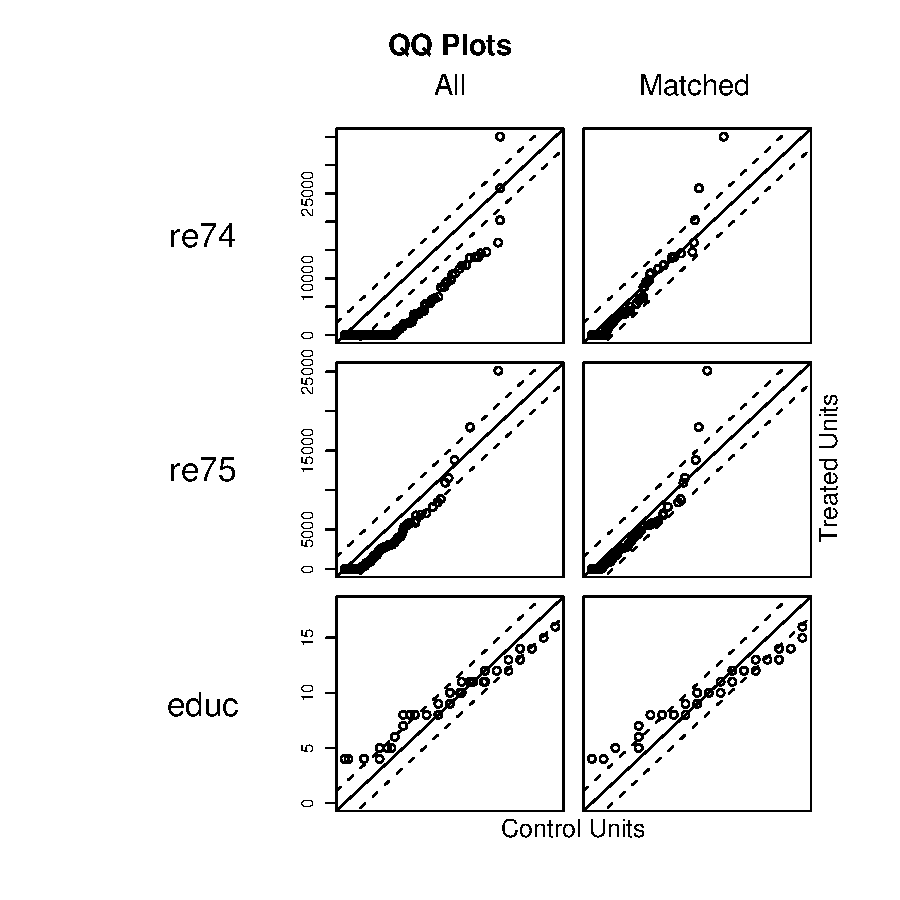
\includegraphics{figs/qqplotnn1}
%    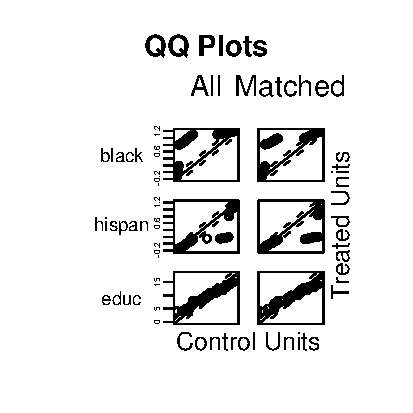
\includegraphics{figs/qqplotnn2}
%    \hfill
%    \caption{Sample diagnostic QQ plots with nearest neighbor matching}
%    \label{diagqqnn}
%  \end{center}
%\end{figure}

%\begin{figure}[tbp]
%  \begin{center}
%    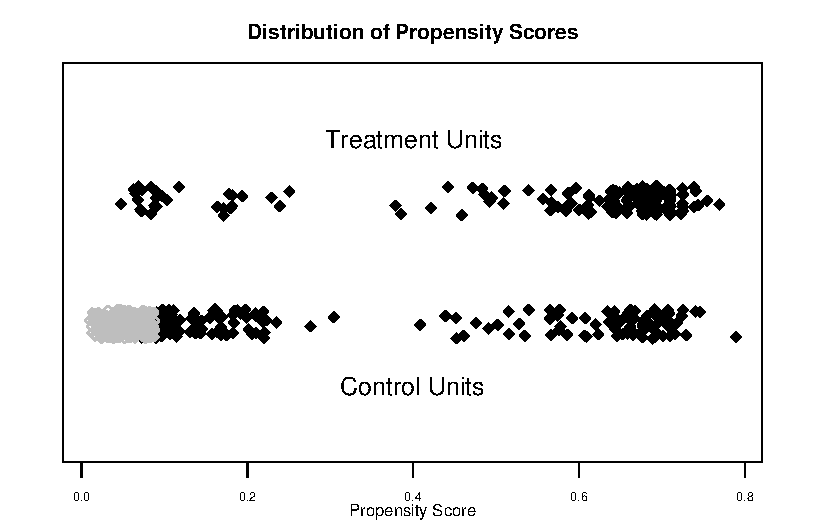
\includegraphics{figs/jitterplotnn}
%    \hfill
%    \caption{Sample diagnostic jitter plot: Matched units shown in
%      black, unmatched units shown in grey.}
%    \label{diagjitternn}
%  \end{center}
%\end{figure}

Two examples of the output from the {\tt plot()} command are shown
below.
%in
%Figures~\ref{diagqqnn}~and~\ref{diagjitternn}. 
The balance of the individual covariates is shown in the Q-Q plots.
If the empirical distributions are the same in the treated and control
groups, the points would all lie on the 45 degree line.  Deviations
from the 45 degree line indicate differences in the empirical
distribution.  The jitter plot shows the overall distribution of
propensity scores in the treated and control groups.  In the jitter
plot, the size of each diamond is proportional to the weight given to
that unit; matched units are in black while unmatched units are in
grey.

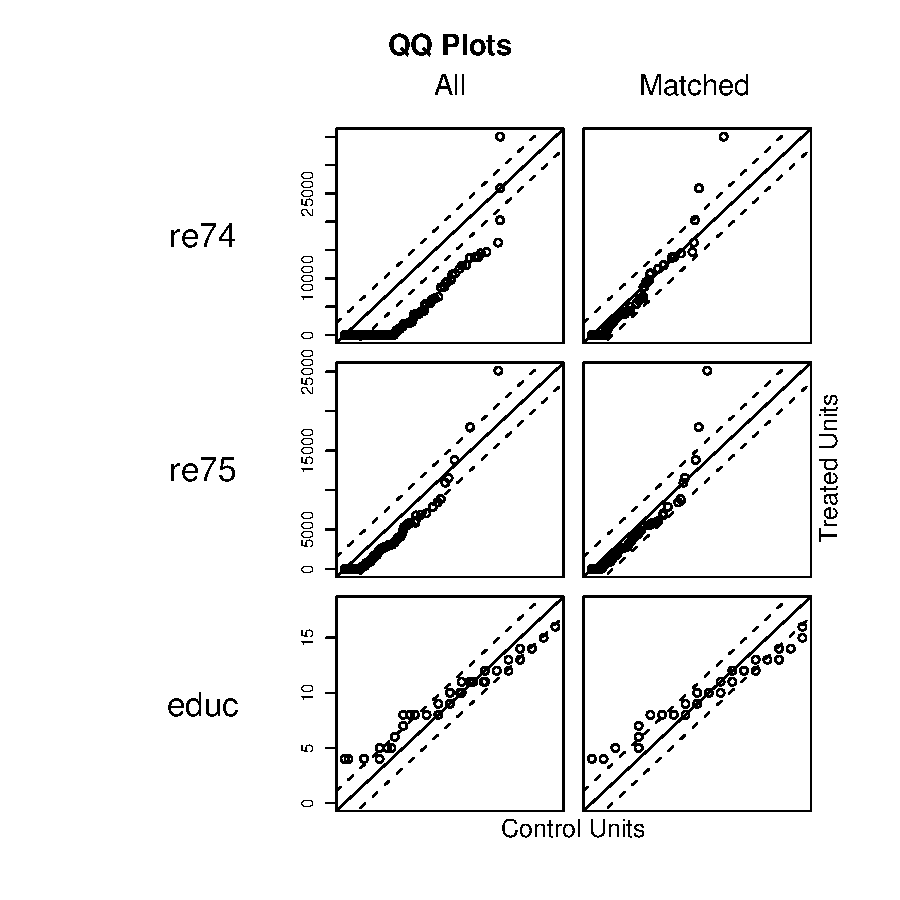
\includegraphics{figs/qqplotnn1}
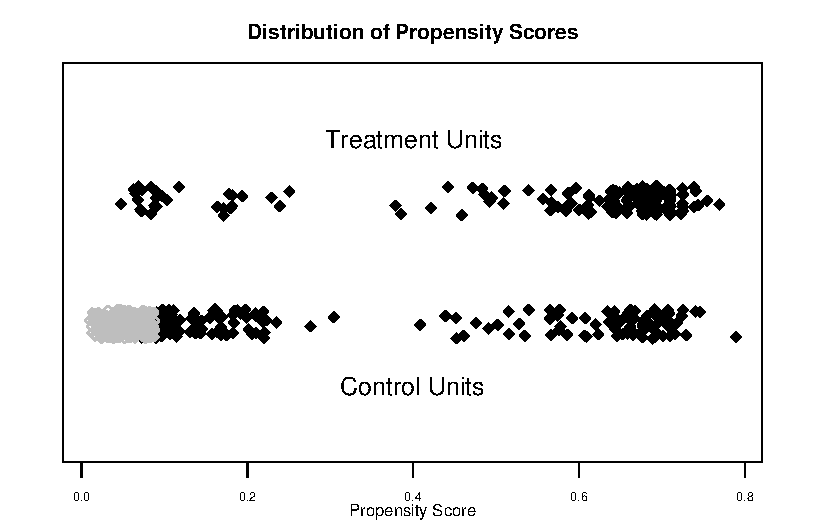
\includegraphics{figs/jitterplotnn}


%%% Local Variables: 
%%% mode: latex
%%% TeX-master: "matchit"
%%% End: 
